\documentclass[a4paper]{article}

%% Language and font encodings
\usepackage[english]{babel}
\usepackage[utf8x]{inputenc}
\usepackage[T1]{fontenc}

%% Sets page size and margins
\usepackage[a4paper,top=3cm,bottom=2cm,left=3cm,right=3cm,marginparwidth=1.75cm]{geometry}

%% Useful packages
\usepackage{amsmath}
\usepackage{graphicx}
\usepackage[colorinlistoftodos]{todonotes}
\usepackage[colorlinks=true, allcolors=blue]{hyperref}

\title{Service-Oriented Architecture}
\author{Keerthana Sanalaprakash \\ Leandre Nzabarushimana \\ Ken Bauwens}

\begin{document}
\maketitle
\pagebreak
\begin{figure}[h]
    \centering
    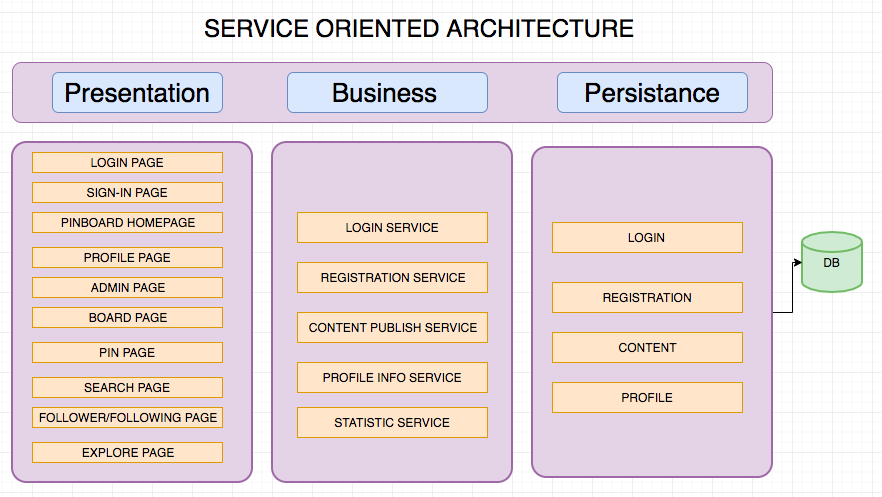
\includegraphics[width=1 \textwidth]{SOA.png}
    \caption{SOA Diagram}
    \label{fig:mesh1}
\end{figure}

\section{Presentation layer}
\textbf{Login page}
\\Page where the user can login using either their own \textit{P4Food} account or their google/facebook account. It will use the login service to validate the login and redirect the user to his pinboard. There will also be an option to create a new account if the user does not already have one.
\\[10px] \textbf{Registration page}
\\Page where the user can create a new \textit{P4Food} account or use google/facebook to create a new account. There will also be an option to login in case the user already has an account. This page will use the registration service to create a new account.
\\[10px] \textbf{Pinboard/Homepage}
\\The landing page which contains the user's followed boards and pins. This page will use the  content service to display the correct pins. 
\\[10px] \textbf{Profile page}
\\Page containing information about a user's profile. This page will use the profile info service to request all the information for a user as well as to update information if the user wants to.
\\[10px] \textbf{Admin page}
\\Page only accessible by admins to see statistics and execute admin commands. This page will only be accessible to admins and will use the statistics service to display the required statistics. An admin can also use the content service to create new categories and remove old ones.
\\[10px] \textbf{Board page}
\\Page where the user can create/update/remove boards. This page will use the content service to display and update the user's boards.
\\[10px] \textbf{Pin page}
\\Page where the user can add/update/remove pins to a specific board. This page will use the content service to display and update the user's pins.
\pagebreak
\\[10px] \textbf{Seach page}
\\The search bar will always be accessible at the top of the page, and the user will be redirected to the search page after he/she searches for something. It will use the content service to find and display relevant search results.
\\[10px] \textbf{Following/Followers page}
\\Page accessible from a user's profile page where  you and other people can see their followers and the people they are following. A user can use these pages to unfollow/block other people. It will use the profile info service to request a user's followers and the users he/she follows.
\\[10px] \textbf{Explore page}
\\Page where users can discover new boards/categories. This page will use the content service to display relevant results.

\section{Logic layer}
\textbf{Login service}
\\Service that handles login requests. It will handle both the \textit{P4Food} accounts and the google/facebook accounts. 
\\[10px] \textbf{Registration service}
\\Service that handles signup requests.  
\\[10px] \textbf{Profile info service}
\\Service that facilitates the retrieval/updating of profile information.
\\[10px] \textbf{Statistics service}
\\Service used by administrators to request statistics like amount of users. Some of the features of this service can be made available through an api for public use.
\\[10px] \textbf{Content service}
\\The service that will facilitate the retrieval/updating/removing of content. Content are boards and pins.

\section{Persistence layer}
\textbf{Login}
\\The server side logic for loging in.
\\[10px] \textbf{Registration}
\\The server side logic for registration.
\\[10px] \textbf{Content}
\\Provide an interface to the database for content activities (boards, pins).
\\[10px] \textbf{Profile}
\\Provide an interface to the database for user information activities.
\end{document}